\documentclass[format=acmlarge,review,natbib]{acmart}

%% Amr
%% words to remember :-)
%% sublime unfathomable
%% ---

% \usepackage{fdsymbol}
\usepackage{bbold}
\usepackage{bussproofs}
\usepackage{keystroke}
\usepackage{comment}
\usepackage{tikz}

%% \usepackage{hyphenat}
%% \usepackage{color}
%% \usepackage{url}
%% \usepackage{amssymb}
%% \usepackage{amsmath}
%% \usepackage{mdwtab}
%% \usepackage{mdwlist}
%% \usepackage{listings}
%% \lstMakeShortInline[columns=fullflexible]|
%% \lstnewenvironment{code}{\lstset{basicstyle={\sffamily\footnotesize}}}{}

\newcommand{\unitepl}{\texttt{unitepl}}
\newcommand{\unitipl}{\texttt{unitipl}}
\newcommand{\unitepr}{\texttt{unitepr}}
\newcommand{\unitipr}{\texttt{unitipr}}
\newcommand{\swap}{\texttt{swap}}
\newcommand{\swapp}{\texttt{swapp}}
\newcommand{\assoclp}{\texttt{assoclp}}
\newcommand{\assocrp}{\texttt{assocrp}}
\newcommand{\unitetl}{\texttt{unitetl}}
\newcommand{\unititl}{\texttt{unititl}}
\newcommand{\unitetr}{\texttt{unitetr}}
\newcommand{\unititr}{\texttt{unititr}}
\newcommand{\swapt}{\texttt{swapt}}
\newcommand{\assoclt}{\texttt{assoclt}}
\newcommand{\assocrt}{\texttt{assocrt}}
\newcommand{\absorbr}{\texttt{absorbr}}
\newcommand{\absorbl}{\texttt{absorbl}}
\newcommand{\factorzr}{\texttt{factorzr}}
\newcommand{\factorzl}{\texttt{factorzl}}
\newcommand{\factor}{\texttt{factor}}
\newcommand{\distl}{\texttt{distl}}
\newcommand{\dist}{\texttt{dist}}
\newcommand{\factorl}{\texttt{factorl}}
\newcommand{\id}{\texttt{id}}
\newcommand{\compc}[2]{#1 \circ #2}
\newcommand{\compcc}[2]{#1 \bullet #2}
\newcommand{\respcomp}[2]{#1 \odot #2}

\newcommand{\Typ}{\mathbf{Type}}
\newcommand{\alt}{~\mid~}
\newcommand{\patht}[1]{\textsc{PATHS}(#1,#1)}
\newcommand{\fpatht}[1]{\textsc{FREEPATHS}(#1,\Box)}
\newcommand{\fpathp}[2]{\textsc{freepath}~#1~#2}
\newcommand{\pathind}[2]{\textsc{pathind}~#1~#2}
\newcommand{\invc}[1]{!\;#1}
\newcommand{\evalone}[2]{eval(#1,#2)}
\newcommand{\evalbone}[2]{evalB(#1,#2)}
\newcommand{\reflp}{\textsc{refl}}
\newcommand{\notp}{\textsc{not}}
\newcommand{\gluep}{\textsc{glue}}
\newcommand{\reflh}{\mathit{refl}_{\sim}}
\newcommand{\symh}[1]{\mathit{sym}_{\sim}~#1}
\newcommand{\transh}[2]{\mathit{trans}_{\sim}~#1~#2}
\newcommand{\reflq}{\mathit{refl}_{\simeq}}
\newcommand{\symq}[1]{\mathit{sym}_{\simeq}~#1}
\newcommand{\transq}[2]{\mathit{trans}_{\simeq}~#1~#2}
\newcommand{\isequiv}[1]{\mathit{isequiv}(#1)}
\newcommand{\idc}{\mathit{id}_{\boolt}}
\newcommand{\swapc}{\mathit{swap}_{\boolt}}
\newcommand{\assocc}{\mathit{assoc}}
\newcommand{\invl}{\mathit{invl}}
\newcommand{\invr}{\mathit{invr}}
\newcommand{\invinv}{\mathit{inv}^2}
\newcommand{\idlc}{\mathit{idl}}
\newcommand{\idrc}{\mathit{idr}}
\newcommand{\swapswap}{\swapc^2}
\newcommand{\compsim}{\compc_{\isotwo}}
\newcommand{\iso}{\leftrightarrow}
\newcommand{\isotwo}{\Leftrightarrow}
\newcommand{\piso}{\multimapdotbothB~~}
\newcommand{\zt}{\mathbb{0}}
\newcommand{\ot}{\mathbb{1}}
\newcommand{\bt}{\mathbb{2}}
\newcommand{\fc}{\mathit{false}}
\newcommand{\tc}{\mathit{true}}
\newcommand{\boolt}{\mathbb{B}}
\newcommand{\univ}{\mathcal{U}}
\newcommand{\uzero}{\mathcal{U}_0}
\newcommand{\uone}{\mathcal{U}_1}
\newcommand{\Rule}[2]{
\makebox{
$\displaystyle
\frac{\begin{array}{l}#1\\\end{array}}
{\begin{array}{l}#2\\\end{array}}$}}
\newcommand{\proves}{\vdash}
\newcommand{\jdgg}[3]{#1 \proves #2 : #3}
\newcommand{\jdg}[2]{\proves #1 : #2}
\newcommand{\jdge}[3]{\proves #1 = #2 : #3}
%% codes
%% denotations

\newcommand{\amr}[1]{\fbox{\begin{minipage}{0.8\textwidth}\color{red}{Amr says: {#1}}\end{minipage}}}


%%%%%%%%%%%%%%%%%%%%%%%%%%%%%%%%%%%%%%%%%%%%%%%%%%%%%%%%%%%%%%%%%%%%%%%%%%%%%%
\begin{document}

\title{Univalent Universes and Completness of Reversible Programs: \\
  Featherweight HoTT}

\author{X}
\affiliation{
  \institution{Y}
  \country{Z}}
\email{A@B.C}

\begin{abstract}
\end{abstract}

\maketitle

%%%%%%%%%%%%%%%%%%%%%%%%%%%%%%%%%%%%%%%%%%%%%%%%%%%%%%%%%%%%%%%%%%%%%%%%%%%%%%
\section{Story and Conjecture}

There is a cottage industry of reversible programming languages, reversible logic, programming applications of type isomorphisms, etc. This work seems it should be connected to HoTT and univalence but there aren't any precise connections or theorems.

Our conjecture:

\begin{itemize}
\item Let $\mathcal{U}$ be the univalent subuniverse generated by $0$, $1$, $+$,
  and $*$ suitably truncated.
\item Let $\Pi$ be the previously  described reversible programming with 1-paths and 2-paths
\item We conjecture that $\Pi$ includes codes for \emph{all} paths in $\mathcal{U}$
\end{itemize}

%%%%%%%%%%%%%%%%%%%%%%%%%%%%%%%%%%%%%%%%%%%%%%%%%%%%%%%%%%%%%%%%%%%%%%%%%%%%%%
\section{Preliminaries}

[Following the HoTT book and the slides on ``A Characterization of Univalent
Fibrations'' by Dan Christensen.]

\paragraph*{Type Family.} A dependent function $P : A \to \mathcal{U}$ defines a
\emph{type family}, $P(x)$ indexed by $x:A$.

\paragraph*{Transport.} Given a type family $P : A \to \mathcal{U}$, a path
$p : x \equiv y$ in $A$ induces a function $p_* : P(x) \to P(y)$ which
transports points in $P(x)$ to points in $P(y)$.

\paragraph*{Fibration.} We think of a type family $P : A \to \mathcal{U}$ as a
\emph{fibration} with base space $A$, with $P(x)$ being the fiber over $x$, and
with $\Sigma_{(x:A)} P(x)$ being the \emph{total space} of the fibration, and
with first projection $\Sigma_{(x:A)} P(x) \to A$. In the figure below, $p_*(u)$
is the transport of $u$ along $p$ and both pairs $(x,u)$ and $(y,p_*(y))$ are in
the total space. A critical property of fibrations is that a path
$p : x \equiv y$ in the base space $A$ and a point $u$ in the fiber over $x$
induce a function that \emph{lifts} the path to the total space: the lifted path
starts at $(x,u)$ and ends at $(y,p_*(u))$. A function $f : \Pi_{(x:A)} P(x)$ is
sometimes called a \emph{section} of the fibration $P$.

\begin{center}
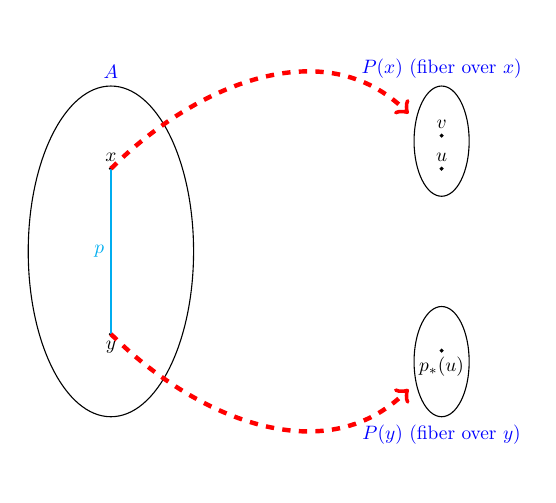
\begin{tikzpicture}[scale=0.7,every node/.style={scale=0.7}]]
  \draw (-3,0) ellipse (1.5cm and 3cm);
  \draw (3,2) ellipse (0.5cm and 1cm);
  \draw (3,-2) ellipse (0.5cm and 1cm);
  \node[blue,ultra thick,above] at (-3,3) {$A$};
  \node[blue,ultra thick,above] at (3,3) {$P(x)$ (fiber over $x$)};
  \node[blue,ultra thick,below] at (3,-3) {$P(y)$ (fiber over $y$)};
  \draw[fill] (-3,1.5) circle [radius=0.025];
  \draw[fill] (-3,-1.5) circle [radius=0.025];
  \draw[left,cyan,thick] (-3,1.5) -- (-3,-1.5);
  \node[above] at (-3,1.5) {$x$};
  \node[below] at (-3,-1.5) {$y$};
  \draw[fill] (3,1.5) circle [radius=0.025];
  \draw[fill] (3,2.1) circle [radius=0.025];
  \draw[fill] (3,-1.8) circle [radius=0.025];
  \node[above] at (3,1.5) {$u$};
  \node[above] at (3,2.1) {$v$};
  \node[below] at (3,-1.8) {$p_*(u)$};
  \node[left,cyan] at (-3,0) {$p$};
  \draw[->,red,dashed,ultra thick] (-3,1.5) to [out=45, in=135] (2.4,2.5);
  \draw[->,red,dashed,ultra thick] (-3,-1.5) to [out=-45, in=-135] (2.4,-2.5);
\end{tikzpicture}
\end{center}

It is worth repeating Remark 2.7.1 from the book. In the figure above, we could
have $(x,u) \equiv (x,v)$ without having $u \equiv v$. The only thing we can
conclude is that there is a (possibly non-trivial) path path $q : x \equiv x$
such that $q_*(u) \equiv v$.

\paragraph*{Univalent Type Family.}
Given standard constructions in the book, we have a function:
\[\begin{array}{rcl}
\textit {transport-equiv} &:& \Pi_{P : A \to \mathcal{U}}~ \Pi_{x,y:A}~
    x \equiv y  \to P x \simeq P y \\
\textit{transport-equiv}~P~x~y &=& \lambda p. \mathit{idtoequiv}(\mathit{ap}_{P}(p))
\end{array}\]
with the standard definitions for
$\mathit{ap} : (x \equiv y) \to (P(x) \equiv P(y))$ and
$\mathit{idtoequiv} : (A \equiv B) \to (A \simeq B)$. We say a type family
$P : A \to \mathcal{U}$ is \emph{univalent} if for all $x,y:A$
the function $\textit{transport-equiv}~P~x~y$ is an equivalence. Formally:
\[\begin{array}{l}
\textit{is-univalent-fibration} : (A \to \mathcal{U}) \to \mathcal{U} \\
\textit{is-univalent-fibration}~P = \Pi_{(x,y:A)} \textit{is-equiv}~(\textit{transport-equiv}~P~x~y)
\end{array}\]

\noindent\paragraph*{Examples}
\begin{itemize}
\item Take $A = \mathcal{U}$ and $P = \mathit{Id}_{\mathcal{U}}$. The statement
  $\textit{is-univalent-fibration}~P$ reduces to $\Pi_{x,y:\mathcal{U}}~x \equiv y \to
  x \simeq y$ which is the usual definition of univalence.

\newpage

\item Take $X = \ot$ with element $\star$ and $P = \lambda \_. \ot$. The
  statement $\textit{is-univalent-fibration}~P$ reduces to
  $(\star\equiv\star)\simeq(\ot\simeq\ot)$ which is true.
\item Take $X = \ot$ and $P = \lambda \_. \zt$. The statement
  $\textit{is-univalent-fibration}~P$ reduces to
  $(\star\equiv\star)\simeq(\zt\simeq\zt)$ which is also true.
\item Take $X = \ot$. For no $P$ other than the above two instances will
  we have a univalent fibration.
\item Take $X = \bt$ with elements $\fc$ and $\tc$ and
  $P = \lambda \_. \ot$. The statement
  $\textit{is-univalent-fibration}~P$ reduces to $(\fc \equiv \tc) \simeq
  (\ot\simeq\ot)$ which is false.
\item Take $X = \bt$ with elements $\fc$ and $\tc$ and
  $P = \lambda \{ \fc \to \zt; \tc \to \ot \}$ The statement
  $\textit{is-univalent-fibration}~P$ reduces to $(\fc \equiv \tc) \simeq
  (\zt\simeq\ot)$ which is true. That is the only choice of $P$
  that works (modulo symmetry).
\item For any $n > 2$, taking $X$ as sum of $n$ copies of $\ot$ can never
  give a univalent fibration.
\end{itemize}

\begin{theorem}
  Let $X$ be path-connected. Then $X$ is the base of a univalent fibration only
  if there exists an $F$ such that $X \simeq \Sigma_{Y : \mathcal{U}} \| Y \equiv F
  \|$. We will refer to this type as $\{F\}$.
\end{theorem}

\noindent In particular $\{\bt\}$, i.e.,
$\Sigma_{Y : \mathcal{U}} \| Y \equiv \bt \|$ is the base of a univalent
fibration. In some sense this is the simplest univalent universe, our
featherweight HoTT that we aim to characterize as a reversible programming
language based on type isomorphisms.

%%%%%%%%%%%%%%%%%%%%%%%%%%%%%%%%%%%%%%%%%%%%%%%%%%%%%%%%%%%%%%%%%%%%%%%%%%%%%%
\section{Some Simple Cases}

Pick $F = \ot$. We have $\{\ot\} \simeq \ot$. Another
simple but less trivial case is $F = S^1$. In that case we also have
$\{S^1\} \simeq S^1$.p

%%%%%%%%%%%%%%%%%%%%%%%%%%%%%%%%%%%%%%%%%%%%%%%%%%%%%%%%%%%%%%%%%%%%%%%%%%%%%%
\section{The Bool Case}

To get started let's look at the case of $\bt$ instead of the entire set of finite types defined using $0$, $1$, $+$, and $*$.

%%%%%
\subsection{$\Pi$}

The restriction of $\Pi$ is the following:

\[\begin{array}{rcl}
\tau &::=& \bt \\
\\
v &::=& \begin{array}[t]{lrcl}
                    & \fc &:& \bt \\
              \alt & \tc &:& \bt
               \end{array} \\
\\
c &::=& \begin{array}[t]{lrcl}
              & \id &:& \tau \iso \tau \\
               \alt & \swap &:& \bt \iso \bt \\
               \alt & \circ &:& (\tau_1 \iso \tau_2) \to (\tau_2 \iso \tau_3)
                              \to (\tau_1 \iso \tau_3)
               \end{array} \\
\\
! &:& (\tau_1 \iso \tau_2) \to (\tau_2 \iso \tau_1) \\
\invc{\id} &=& \id \\
\invc{\swap} &=& \swap \\
\invc{(\compc{c_1}{c_2})} &=& \compc{\invc{c_2}\;}{\;\invc{c_1}} \\
\\
\alpha &::=& \begin{array}[t]{lrcl}
               & \id &:& c \isotwo c \\
               \alt & \assocc &:& \compc{c_1}{(\compc{c_2}{c_3})} \isotwo
                                              \compc{(\compc{c_1}{c_2})}{c_3} \\
               \alt & \idlc &:& \compc{\id}{c} \isotwo c \\
               \alt & \idrc &:& \compc{c}{\id} \isotwo c \\
               \alt & \invl &:& \compc{c\;}{\;\invc{c}} \isotwo \id \\
               \alt & \invr &:& \compc{\invc{c}}{c} \isotwo \id \\
               \alt & \bullet &:& (c_1 \isotwo c_2) \to (c_2 \isotwo c_3)
                                            \to (c_1 \isotwo c_3) \\
               \alt & \odot &:& (c_1 \isotwo c_1') \to (c_2 \isotwo c_2')
                                            \to (\compc{c_1}{c_2} \isotwo \compc{c_1'}{c_2'}) \\
             \end{array}
\end{array}\]

The 2-combinators $\alpha$ also have inverses. The above forms a 2-groupoid (see
accompanying code once it is fixed).

%%%%%
\subsection{$\mathcal{U}$}

We assume an ambient univalent universe defined like in the HoTT book and including dependent pairs, a unit type, coproducts, identity types, and constants $\textsc{funext}$ and $\textsc{univalence}$. Our universe $\mathcal{U}$ is the subuniverse of this ambient universe defined as $\Sigma_{X:\mathbf{Type}} \| X \equiv \bt \|$ where:

\begin{itemize}

\item $\Sigma$ is the type former for dependent pairs: it comes equipped with an introduction rule, an induction principle, and a computational rule.

\item $\bt$ is the type of booleans which comes with the two points, an induction principle, and computational rules.

\item $\equiv$ is the identity type former which comes with $\reflp$, an induction principle $J$, and a computation rule.

\item $\| A \|$ is the propositional truncation of $A$ defined as follows: for
  any $x:A$ we have $|x| : \|A\|$, and for any $x,y : \|A\|$, we have
  $\gluep : x \equiv y$.

\end{itemize}

%%%%%
\subsection{Equivalence}

Now we claim that $\mathcal{U}_\Pi$ is equivalent to $\mathcal{U}$ where
$\mathcal{U}_\Pi$ is a universe which includes types $\tau$ as a points,
combinators $c : \tau_1 \iso \tau_2$ as 1-paths, and 2-combinators
$\alpha : c_1 \isotwo c_2$ as 2-paths. The proof is in a meta-logic which is
itself univalent.

We begin by unpacking the objects, 1-paths, and 2-paths of $\{\bt\}$.

\paragraph*{Objects in $\{\bt\}$.} The only term in $\{\bt\}$ is
$(\bt,\|\reflp_{\bt}\|)$ which we call $`\bt$. Formally we can prove
$\|(X,p) \equiv `\bt\|$ is inhabited for all $X$ and $p$.

\paragraph*{1-Paths in $\{\bt\}$.} These are paths between $`\bt$ and
$`\bt$. Generally speaking, paths between elements of a $\Sigma$-type are pairs
of paths with a transport in the second component. If we have a type $A$ with
points $a$ and $b$ and a path $p : a \equiv b$. Fix some $c$ and consider the
dependent function $(x:A) \rightarrow (x \equiv c)$. This forms the types
$a\equiv c$ and $b\equiv c$ with elements $ua$ and $ub$. Now a path between
$(a,ua)$ and $(b,ub)$ is a pair $(p,\alpha)$ where $\alpha : p_* ua \equiv
ub$. Hence paths between $`\bt$ and $`\bt$ are going to be for the form
$(p,\alpha)$ where $p : \bt \equiv \bt$ and $\alpha$ is essentially $\gluep$
from the definition of truncation. So we have two paths:
\[\begin{array}{rcl}
`\mathbf{id} &=& (\reflp,\gluep) \\
`\mathbf{not} &=& (\notp,\gluep)
\end{array}\]

\paragraph*{2-Paths in $\{\bt\}$.} Now are considering paths between
$`\mathbf{id}$ and $`\mathbf{id}$, and between $`\mathbf{not}$ and
$`\mathbf{not}$. We have at least one path at this level which is
$(\reflp,\gluep)$ but to show that that this is the only path we will have to
first prove that $`\mathbf{not} \circ `\mathbf{not} \equiv `\mathbf{id}$.

%%%%%%%%%%%%%%%%%%%%%%%%%%%%%%%%%%%%%%%%%%%%%%%%%%%%%%%%%%%%%%%%%%%%%
%%%%%%%%%
\section{Generalization I}

Use all finite types instead of just Bool

%%%%%%%%%%%%%%%%%%%%%%%%%%%%%%%%%%%%%%%%%%%%%%%%%%%%%%%%%%%%%%%%%%%%%
%%%%%%%%%
\section{Generalization II}

Add a HIT to the univalent universe, perhaps something to do with fractionals.


%%%%%%%%%%%%%%%%%%%%%%%%%%%%%%%%%%%%%%%%%%%%%%%%%%%%%%%%%%%%%%%%%%%%%%%%%%%%%%
\bibliographystyle{acm}
{\footnotesize
\bibliography{cites}
}
\end{document}
